
\chapter{Hash table}

\keyword{Hash Table} is a data structure which organizes data using hash functions in order to support quick insertion and search.

There are two different kinds of hash tables:
\begin{description}
\item[hash set] The hash set is one of the implementations of a set data structure to store no repeated values.
\item[hash map] The hash map is one of the implementations of a map data structure to store (key, value) pairs.
\end{description}

\section{The principle of hash table}

The key idea of Hash Table is to use a \keyword{hash function} to map \keyword{keys} to \keyword{buckets}. To be more specific,
\begin{enumerate}
\item When we insert a new key, the hash function will decide which bucket the key should be assigned and the key will be stored in the corresponding bucket;
\item When we want to search for a key, the hash table will use the same hash function to find the corresponding bucket and search only in the specific bucket.
\end{enumerate}


\section{Keys to design a hash table}

There are two essential factors that you should pay attention to when you are going to design a hash table.

\subsection{Hash function}

The hash function is the most important component of a hash table which is used to map the key to a specific bucket.
The hash function will depend on the \keyword{range of key values} and the \keyword{number of buckets}.


It is an open problem to design a hash function.
The idea is to try to assign the key to the bucket \keyword{as uniform as you can}.
Ideally, a perfect hash function will be a one-one mapping between the key and the bucket.
However, in most cases a hash function is not perfect and it is a tradeoff between \keyword{the amount of buckets} and \keyword{the capacity of a bucket}.


\subsection{Collision resolution}

Ideally, if our hash function is a perfect one-one mapping, we will not need to handle collisions.
Unfortunately, in most cases, collisions are almost inevitable.
For instance, hash function (y = x \% 5), both 1987 and 2 are assigned to bucket 2.
That is a \keyword{collision}.


A collision resolution algorithm should solve the following questions:

\begin{enumerate}
\item How to organize the values in the same bucket?
\item What if too many values are assigned to the same bucket?
\item How to search a target value in a specific bucket?
\end{enumerate}

These questions are related to \keyword{the capacity of the bucket} and \keyword{the number of keys} which might be mapped into \keyword{the same bucket} according to our hash function.

Let's assume that the bucket, which holds the maximum number of keys, has N keys.

Typically, if N is constant and small, we can simply use an array to store keys in the same bucket. If N is variable or large, we might need to use height-balanced binary search tree instead.



\section{The principle of built-in hash table}

The typical design of built-in hash table is:
\begin{enumerate}
\item The key can be any \keyword{hashable} type. And a key with belongs to a hashable type will have a \keyword{hashcode}. This code will be used in the mapping function to get the bucket index.
\item Each bucket contains \keyword{an array} to store all the values in the same bucket initially.
\item If there are two many values the same bucket, these values will be maintained in a \keyword{height-balanced binary search tree} instead.
\end{enumerate}

The average time complexity of both insertion and search is still \keyword{O(1)}.
And the time complexity in the worst case is \keyword{O(logN)} for both insertion and search by using height-balanced BST.



\section{Designing the key}

Sometimes you have to think it over to design a suitable key when using a hash table.

For example:
\begin{tcolorbox}
\begin{verbatim}
Given an array of strings, group anagrams together.
\end{verbatim}  
\end{tcolorbox}


As we know, a hash map can perform really well in grouping information by key.
But we cannot use the original string as key directly.
We have to design a proper key to present the type of anagrams.
For instance, there are two strings "eat" and "ate" which should be in the same group.
While "eat" and "act" should not be grouped together.


When you design a key, you need to guarantee that:
\begin{enumerate}
\item All values belong to the same group will be mapped in the same group.
\item Values which needed to be separated into different groups will not be mapped into the same group.
\end{enumerate}


This process is similar to design a hash function, but here is an essential difference.
A hash function satisfies the first rule but might not satisfy the second one.
But your mapping function should satisfy both of them.




\subsection{Summary}

Here are some takeaways about how to design the key for you:
\begin{enumerate}
\item When the order of each element in the string/array doesn't matter, you can use the \keyword{sorted string/array} as the key.
\item If you only care about the offset of each value, usually the offset from the first value, you can use the \keyword{offset} as the key.
\item In a tree, you might want to directly use the \keyword{TreeNode} as key sometimes. But in most cases, the \keyword{serialization of the subtree} might be a better idea.
\item In a matrix, you might want to use \keyword{the row index} or \keyword{the column index} as key.
\item In a Sudoku, you can combine the row index and the column index to identify which \keyword{block} this element blongs to.
\item Sometimes, in a matrix, you might want to aggregate the values in the same \keyword{diagonal line}. $(i,j) \rightarrow i+j$, $(i,j) \rightarrow i-j$
\end{enumerate}



\section{Conclusion}

A typical thinking process to solve problems by hash table flexibly show in Figure \ref{fig:how-to-apply-hash-table}:
\begin{figure}[!ht]
  \centering
  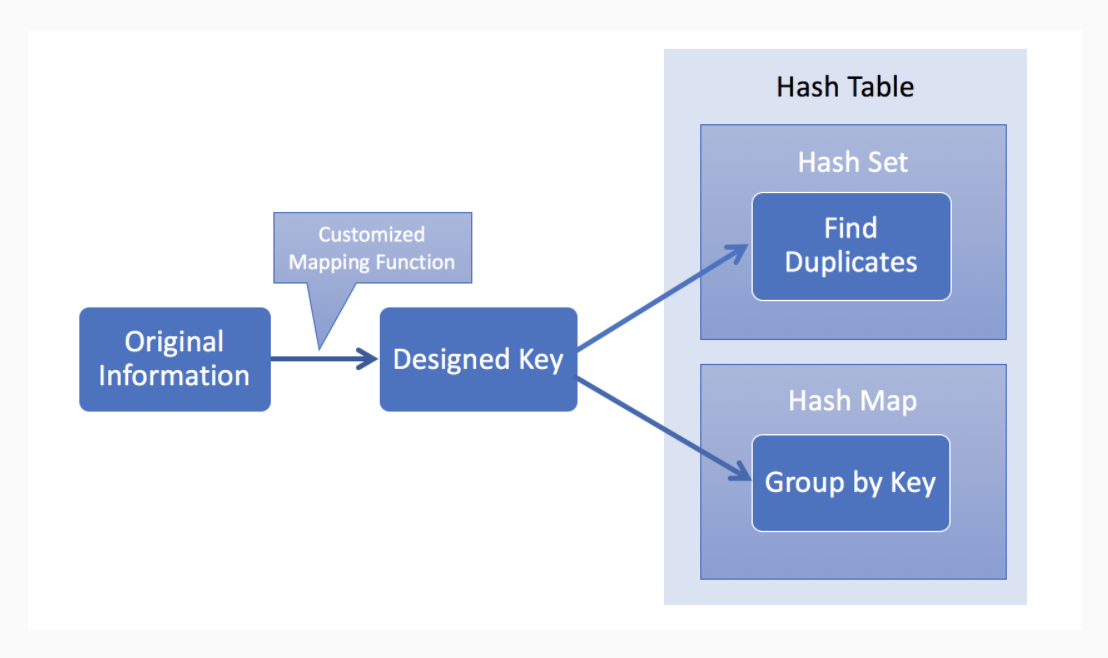
\includegraphics[width=\textwidth]{pics/how-to-apply-hash-table}
  \caption{Thinking process by hash table}
  \label{fig:how-to-apply-hash-table}
\end{figure}



What's more, we will meet more complicated problems sometimes. We might need to:

\begin{itemize}
\item use several hash tables together
\item combine the hash table with other data structure
\item combine the hash table with other algorithms
\item ...
\end{itemize}
